%%%%%%%%%%%%%%%%%%% author.tex %%%%%%%%%%%%%%%%%%%%%%%%%%%%%%%%%%%
%
% sample root file for your "contribution" to a contributed volume
%
% Use this file as a template for your own input.
%
%%%%%%%%%%%%%%%% Springer %%%%%%%%%%%%%%%%%%%%%%%%%%%%%%%%%%


% RECOMMENDED %%%%%%%%%%%%%%%%%%%%%%%%%%%%%%%%%%%%%%%%%%%%%%%%%%%
\documentclass[graybox]{svmult}

% choose options for [] as required from the list
% in the Reference Guide

\usepackage{mathptmx}       % selects Times Roman as basic font
\usepackage{helvet}         % selects Helvetica as sans-serif font
\usepackage{courier}        % selects Courier as typewriter font
\usepackage{type1cm}        % activate if the above 3 fonts are
                            % not available on your system
%
\usepackage{makeidx}         % allows index generation
\usepackage{graphicx}        % standard LaTeX graphics tool
                             % when including figure files
\usepackage{multicol}        % used for the two-column index
\usepackage[bottom]{footmisc}% places footnotes at page bottom
% see the list of further useful packages
% in the Reference Guide

\makeindex             % used for the subject index
                       % please use the style svind.ist with
                       % your makeindex program

%%%%%%%%%%%%%%%%%%%%%%%%%%%%%%%%%%%%%%%%%%%%%%%%%%%%%%%%%%%%%%%%%%%%%%%%%%%%%%%%%%%%%%%%%

\begin{document}

\title*{Predication Instances spot price in EC2}
\author{test test}
\institute{Name of First Author \at Name, Address of Institute, \email{name@email.address}
\and Name of Second Author \at Name, Address of Institute \email{name@email.address}}
%
% Use the package "url.sty" to avoid
% problems with special characters
% used in your e-mail or web address
%
\maketitle

\abstract{We analyze G2 spot instance price}

\section{Introduction}\label{sec:1}



In this paper, we focus to analyze the predication of spot instances price for 7 regions by use different time series models such as ARIMA, SARIMA VAR, DLM, prophet, average and naïve model
our work covered  7 regions of spot instances datasets, ap-northeast-1, ap-southeast-1, ap-regions, and 5 types and different period of datasets G2(03-02 to 2016-10-31),I2(2016-05-03 to 2017-02-04),M4,c3,R3(2016-03-02 to 2017-02-04)








Explain opportunistic cloud computing resources with spot instance in EC2

Mention the difficulies of price change prediction
Ben-Yehuda et. al~\cite{spot-instance-pricing-analysis}

Describe uniqueness of GPU spot instance with DeepSpotCloud

Summarize the overall contents

\section{Time-Series Analysis for GPU Spot Instances}
List basic methods that are widely used in other wors

naive

mean

seasonal mean

ARIMA with different parameters 
stander for Autoregressive Integrated Moving Average, which is the most popular statistical model and widely used to forecasting a time series, the model is a combination of  autoregressive Eq.~\ref{Eq-AR} and moving-average model Eq.~\ref{Eq-MA}, with three parameters  (p,d,q) where p is the number of autoregressive terms, which is depends on past values, d is the degree of differencing and q is the number of lagged forecast errors in the prediction equation, depends only on the random error terms 
\begin{equation}
 y_t = w_0 +\beta_1 y_{t-1}+ \beta_2 y_{t-2}+.....\beta_n y_{t-n}+\epsilon_t
\label{Eq-AR}
\end{equation}


\begin{equation}
 y_t = w_0 +\epsilon_t + \delta_1 \epsilon_{t-1}+  \delta_2 \epsilon_{t-2}+...+ \delta_n \epsilon_{t-n}
\label{Eq-MA}
\end{equation}

Thus, ARIMA if d=n will be 
\begin{equation}
 y_t = w_0 +\beta_1 y_{t-1}+ \beta_2 y_{t-2}+.....\beta_n y_{t-n} +  \delta_1 \epsilon_{t-1}+  \delta_2 \epsilon_{t-2}+...+ \delta_n \epsilon_{t-n}+
\label{Eq-ARIMA}
\end{equation}
Where the term \(\beta_i \) is, weight applied to prior values in the time series \(\delta_i \) is autocorrelation coefficients at lags and \(\epsilon_i \) is residual error term 
\section{Evaluation}
Compare all the methods of different types of algorithms to different instance types
\begin{figure}
\centering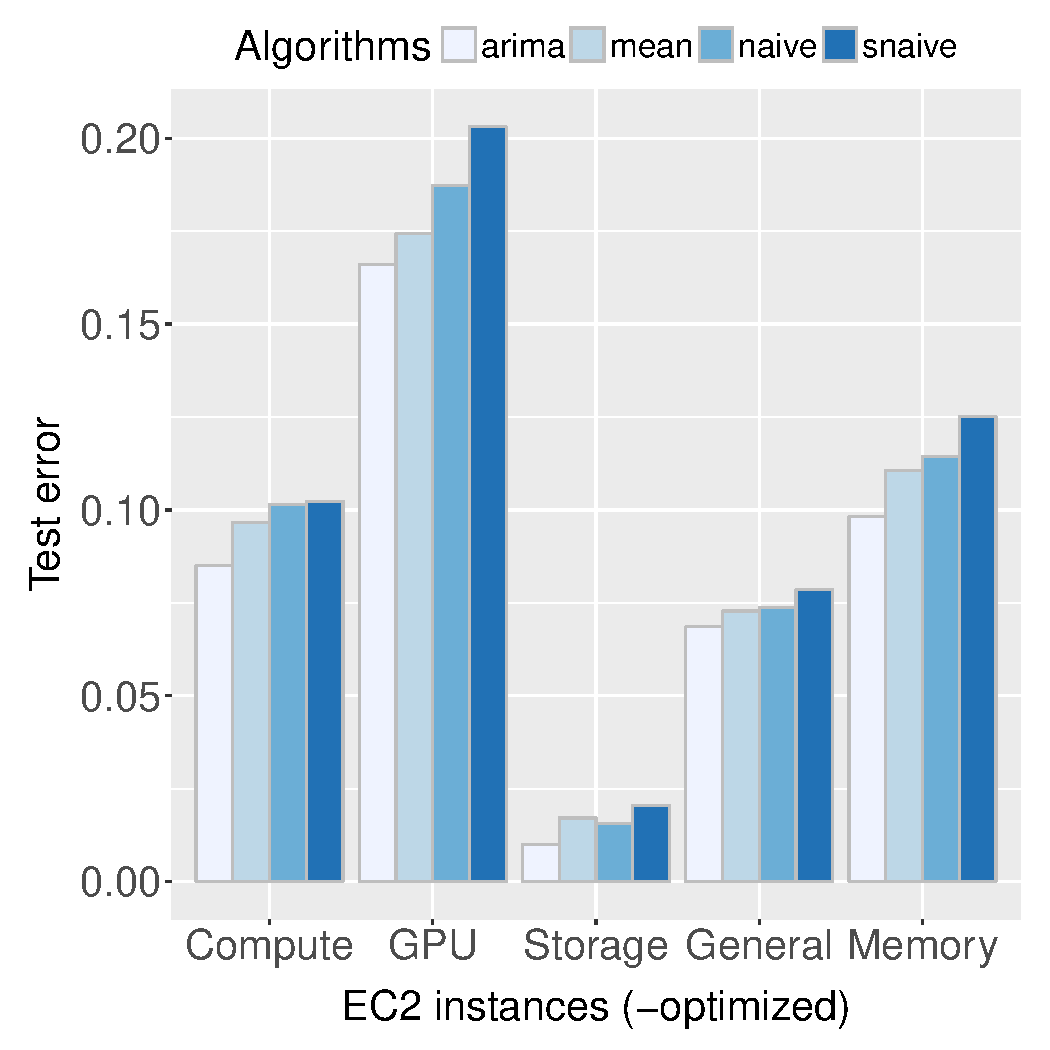
\includegraphics[width=0.7\textwidth]{figures/algorithm-compare-different-instance-type.pdf}\caption{Algorithms with different instance types\label{fig:algo-diff-inst}}
\end{figure}

\section{Conclusion}
Summarize

\begin{acknowledgement}
Thanks to ...
\end{acknowledgement}
\bibliographystyle{spmpsci}
\bibliography{g2-price-modeling}
\end{document}
